\documentclass[11pt]{article}
\usepackage[left=2cm,top=2cm,right=2cm,bottom=2cm]{geometry}
\geometry{letterpaper}                   % ... or a4paper or a5paper or ... 
%\geometry{landscape}                % Activate for for rotated page geometry
%\usepackage[parfill]{parskip}    % Activate to begin paragraphs with an empty line rather than an indent
\usepackage{graphicx}
\usepackage{amsmath}
\usepackage{amsfonts}
\usepackage{amssymb}
\usepackage{epstopdf}
\usepackage{ulem}
\usepackage[draft]{pdfpages}
\DeclareGraphicsRule{.tif}{png}{.png}{`convert #1 `dirname #1`/`basename #1 .tif`.png}
\def \dbar{{\mathchar'26\mkern-12mu d}}
\newcommand{\kB}{k_{\mathrm{B}}}
\newcommand{\traj}{\text{traj}}
\newcommand{\ee}{\mathrm{e}}
\newcommand{\tobs}{t_\mathrm{obs}}
\newcommand{\eps}{\epsilon}
\newcommand{\sig}{\sigma}
\newcommand{\ii}{\mathrm{i}}
\newcommand{\CC}{\mathcal{C}}
\newcommand{\WW}{\mathbb{W}}
\newcommand{\HH}{\mathbb{H}}
\newcommand{\EE}{\mathbb{E}}
\newcommand{\FF}{\mathcal{F}}

\newcommand{\rate}{\lambda}
\newcommand{\upr}{\gamma}

\newcommand{\zz}{\ee^{-s}}
\newcommand{\zzs}{\ee^{-s^*}}

\newcommand{\Sc}{S}

\renewcommand{\figurename}{\textbf{Figure}}

% Different font in captions
\newcommand{\captionfonts}{\small}

\makeatletter  % Allow the use of @ in command names
\long\def\@makecaption#1#2{%
  \vskip\abovecaptionskip
  \sbox\@tempboxa{{\captionfonts #1: #2}}%
  \ifdim \wd\@tempboxa >\hsize
    {\captionfonts #1: #2\par}
  \else
    \hbox to\hsize{\hfil\box\@tempboxa\hfil}%
  \fi
  \vskip\belowcaptionskip}
\makeatother   % Cancel the effect of \makeatletter

\renewcommand{\abstractname}{Summary}

 \def\dsp{\def\baselinestretch{2.0}\large\normalsize}
%\dsp

\title{{Out of equilibrium dynamical systems, the path from A to B.}}
\author{Yael S. Elmatad}
\date{}                                           % Activate to display a given date or no date
\begin{document}
\maketitle
%\section{}
%\subsection{}
%\includepdf[pages=-]{pdfpages.pdf}
%\section{Long-Term Objectives}
\begin{abstract}
Increasingly, statistical physics has had to grapple with a new set of scientific questions in which techniques of classical, equilibrium thermodynamics have to be stretched in order to apply to inherently slow, out-of-equilibrium, and often driven systems.   As these systems are out-of-equilibrium, it does not suffice to simply study ensembles of configurations. Instead, we are forced to examine dynamical ensembles of trajectories.  One such problem is that of glass transition.  Reconciling the apparent disparity between the microscopic, disordered nature of glass and its macroscopic rigidity has confounded physicists for years. However, we have recently shown how studying a simple model in trajectory space can shed light on the true nature and universality of molecular glassformers. I propose to further this work not only to continue my study of glasses but also to extend the methods developed to study these slow systems to other systems such as the biophysical problem of crowded cellular environments.  Beyond these applications, I also propose to extend the dynamical sampling methods even further, thus allowing us to not only learn more information about the physical world we live in but also gain new ways to engineer models and novel materials to preform desired behaviors


%Increasingly, statistical physics has had to grapple with a new set of scientific questions where techniques of classical, equilibrium thermodynamics have to be stretched to inherently slow, out-of-equilibrium, and sometimes driven systems.  Since these systems are out-of-equilibrium it does not suffice to simply study ensembles of configurations, instead, we are forced to examine dynamical ensembles of trajectories.  One such problem is the problem of the glass transition.  Reconciling the apparent disparity between the microscopic, disordered nature of glass and its macroscopic rigidity has confounded physicists for years. However, we have recently shown how studying a simple model in trajectory space can shed light on the true nature and universality of molecular glassformers. In this statement I propose to further this work not only to continue my study of glasses but also to extend the methods developed to study these slow systems to other systems such as the biophysical problem of crowded cellular environments.  Beyond applications, I propose to extend the dynamical sampling methods even further, thus allowing us to not only learn more information about the physical world we live in but also gain new ways to engineer models and novel materials to preform desired behaviors.

%Glassy materials have wide ranges of applications, including nuclear storage~\cite{Sales1984}, cryobiology~\cite{Lemler2004}, and pharmaceuticals~\cite{Craig1999}. Understanding glassy phenomena would lead to advancements in these fields, such as extending the life of organs for transplant~\cite{Lemler2004} and improving the safe long-term storage of nuclear waste~\cite{Sales1984}.  However, a strong impediment to the effective design of glassy materials with desired properties is the lack of a detailed understanding of the very nature of the glass transition, and whether it is thermodynamic or kinetic in origin. Our earlier work, utilizing an advanced trajectory sampling technique called transition path sampling (TPS)~\cite{Bolhuis_AnnuRevPhysChem_2002}, has taught us a great deal about the origin of the glass transition in model glass formers. However, new techniques are still needed to improve the sampling of realistic glass models as well as to design new materials that are glassy~\cite{Whitesides2002}. Current methods involve scanning parameter space by trial and error and conducting long, time-consuming simulations of material formation for each trial parameter set. Here, I propose a method which optimizes parameters for a given model based on path probabilities for a transition path ensemble.  This method circumvents these problems by making forays in thermodynamic parameter space and extends the technique of parallel tempering to allow for sampling in both trajectory and parameter space.  These techniques will also facilitate the engineering of synthetic self-assembling nanomaterials, which have applications to drug delivery~\cite{Rosler2001} and new materials~\cite{Whitesides2002}.   Moreover, I believe these methods have wide applicability to related sampling and optimization problems.
\end{abstract}

%\section*{Aims}
\section{The Glass Transition}
Supercooled liquids and the glass transition are a much debated and poorly understood physical phenomenon.  The nature of supercooled liquids is inherently out of equilibrium as the equilibrium state (crystalline solid) is avoided by a slow cooling protocol that frustrates the previously in-equilibrium liquid.  In recent work, we have shown how it is possible to take a wide range of experimental data for  molecular glass former transport properties and collapse them onto a single curve. Many of the data taken on supercooled liquids originate from measurements that involve probe particles - guest particles that are used as `thermometers' for their host liquid which can be used as recorders of transport properties as well as dynamic heterogeneity.  One behavior that has yet to be fully understood is to what extent these probes can record useful information about their host solvents.  Conventionally, probe particles are made to be as ``inconspicuous" as possible to mimic the behavior of the host.  I would like to investigate how far this can be pushed.  For example, can the probe size be swelled until the probe is on the order of the size of dynamic heterogeneities.   Once the probe size is of that order it should recover the mean field behavior of an average liquid -- for example, the diffusion constant and the relaxation time should be coupled as per the Stokes-Einstein equation, even when the host supercooled liquid shows decoupling. I intend to study the effects of probe particles on host liquids by use of molecular dynamics and Monte-Carlo simulations of glass-formers.  Through these studies, it can be understood to what extent the probe particle can be used as a molecular thermometer for the host and, moreover, to what extent and in what regime does the probe actually disturb the normal dynamics of the host liquid.  These insights are useful to experimentalist who often assume that the probe acts only as a `passive' recorder of the host solvent's dynamics.  The extent to which this assumption is valid, is something that should be further tested.

\section{Crowded Environments}
Recently, many have touted the analogy between crowded cellular environments and the colloidal glass transition.  By increasing the osmotic pressure inside a cell, experimenters were able to `jam' the interior environment, just as they would a dense colloidal or granular material.  While this pressure was applied in a laboratory, this increase in pressure is also felt during rapid tumor formation as cells become more and more densely packed due to rapidly dividing cells.  Since cells are crowded out of equilibrium environments they share many features with supercooled liquids -- also dense packings of molecules, only on a different scale.  Recent numerical work and simulation technique advances have been used to shed light on elementary motion in such supercooled environments.  By exploiting the similarity, large molecular simulations of a dense cellular work coupled with new techniques can be used to further study basic motion of small proteins as they diffuse in such a crowded environment.  These simulations would use techniques of transition path sampling to characterize the ensemble of possible moves as a protein escapes its environment by exiting its cage.  Questions about the nature of these motions -- and to what extend they resemble the facilitated motions in granular and colloidal materials -- would help us understand the physical environment of the biological material that makes up a cell. 

Intracellular materials are not the only biological system with analogies with jammed materials.  Recent work in microfluidic devices have shown how sickle-cell disease manifests itself when cells change their shape and form clots is small chambers (veins).  The geometry of the cells as they ``sickle" has been shown to play an important role in acute attacks of the disease.  Understanding basic elementary processes about how clots form and break apart can be of use to creating new treatment for the disease.  For example, it has been shown that a small molecular inhibitor can be used to break up such clots, however that inhibitor was carbon monoxide -- a toxic chemical.  Molecular simulation may be useful in understanding what kind of guest molecules would be best at preventing and treating these clots.  Perhaps by elucidating which size and shape molecules can be used to frustrate the formation of such clots.  Again being able to single out elementary steps using transition path sampling techniques will help elucidate the key steps to the formation and destruction of such clots.

\section{Sampling Methods}

In a recent interview, when asked what the greatest challenges for computational materials science is, pioneering researcher Michele Parrinello stated that ``...sampling is really the most important aspect to be improved...''.
% \cite{Parrinello2010}.
To that end, I will develop methods to improve sampling and design in materials.  The first aim of this work is to use a new parameter space sampling technique to investigate ensembles of trajectories.  This method would investigate rare events in complex dynamical systems with increased computational efficiency. The second aim is to use a novel method to optimize parameters to select for a certain dynamical behavior.  This second technique would allow us to engineer models which strike a balance between thermodynamics and dynamics.  Both methods have applications for studying glass formers, biophysics, and designing novel materials.

%\section*{Background and Significance}

%\subsection*{Glassy behavior is a ubiquitous phenomenon with wide applicability}
%Glasses are formed when liquids are supercooled beyond their freezing temperature rapidly enough to avoid crystal formation, forming a ``metastable" but long lived state that preserves the liquid structure \cite{Ediger1996, Angell_Science_1995}.   Understanding the apparent disconnect between the macroscopic solid-like properties of a glass and the microscopic liquid-like properties has, however, eluded glass physicists for some time. Such an understanding of glassy phenomena is essential because it has applications to not only material science \cite{Schulli2010} but also has been recently implicated in a wide variety of processes such as jamming in granular material \cite{Clusel2009}, biological cells under compression \cite{Zhou2009}, and protein folding \cite{Gin2009}. Glasses can be used as a means for nuclear waste storage \cite{Sales1984} as well as for making pharmaceuticals more shelf-stable \cite{Craig1999}. One of the most polarizing debates surrounding glasses has concerned the importance of dynamics compared to thermodynamics in glass formers.  There are many who purport that glassy behavior is entirely thermodynamic \cite{Lubchenko_AnnuRevPhysChem_May_2007}. Others, however, have contended that it is a purely dynamic phenomenon \cite{Garrahan2003}.

%\subsection*{Kinetically constrained models capture glassy dynamic heterogeneity}
%To investigate the dynamics of glass formers, my colleagues and I have been studying kinetically constrained models (KCMs) such as the Fredrickson-Andersen model (FA) \cite{Fredrickson_PhysRevLet_Sept_1984} .  This class of models is motivated by experiments of glass formers showing that glassy systems experience dynamic heterogeneity: that some regions of glass formers relax faster than others \cite{Ediger1996, Angell_Science_1995}.  These dynamic heterogeneities have been linked to a phenomenon known as facilitation. An excitation is thought by many to be the mechanism by which supercooled liquids relax. As an excitation travels through the system it brings local mobility to the region.  A region is more likely to become mobile itself if a neighboring region has been recently active, thus mobility is facilitated by neighboring sites \cite{Keys_NatPhys_Apr_2007}.  Moreover, we have shown glass universality in experimental systems using a theory derived from KCMs by showing that relaxation times for over 50 glass formers collapse to a single curve, thus supporting the idea that kinetic effects dominate glassy behavior \cite{Elmatad2009}. KCMs are models whose underlying thermodynamics are very simple, but whose glassy behavior is due to a purely kinetic constraint.  In the case of the FA model it is just that of a 1 dimensional lattice gas (non-interacting spins on a lattice) \cite{IMSM}. Facilitation is added through a kinetic constraint.

%\subsection*{Ensembles of trajectories using Transition showcase the nature of Kinetically Constrained Models}
%Using simple models for glassformers known as kinetically constrained models (KCMs), we previously studied the dynamical ensemble (i.e., the ensemble of trajectories) rather than a static ensemble (i.e., the ensemble of configurations).  We found that this model undergoes a dynamic first-order phase transition. That is, there is a discontinuity in an order parameter, $K$, which measures the ``activity'' in the model (in our case, the number of configuration changes) which is coupled to a dynamical field $s$.  This behavior was qualitatively demonstrated for atomistic models \cite{Hedges_Science_2009} as well.  Upon mild constraint softening, the first-order dynamical phase transition does persist, though eventually the system goes through a critical point and then finally into a one-phase region which approaches a lattice gas \cite{Elmatad_PNAS_2010}.  This dynamical phase transition is highlighted in Figure \ref{fig:softFA} alongside a phase diagram in the $s$ and $\epsilon$ plane. $\epsilon$ is the measure of ``softness'': $\epsilon=0$ is the pure FA model and $\epsilon \rightarrow \infty$ recovers the lattice gas. 

%\begin{figure}[b!] %  figure placement: here, top, bottom, or page
%   \centering
 %  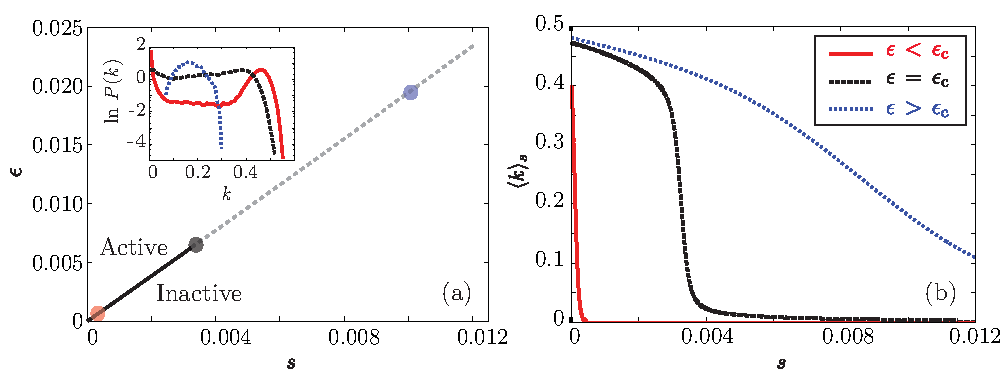
\includegraphics[width=5in]{softFA.pdf} 
 %  \caption{Example of a dynamical phase transition in the soft FA model. $\langle k \rangle_{s}$ is the intensive equivalent of $K$, where $k$ is the activity per space-time unit volume.  (a) shows the phase diagram in the $\epsilon$, $s$ plane.  Inset shows the probability distribution at a value of $s$ indicated by the dots in the phase diagram. (b) shows $\langle k \rangle_{s}$ as a function of $s$ at the same state points as the inset of (a) and the dots indicated in (a).  Labeling and colors are the same throughout.  For more, see \cite{Elmatad_PNAS_2010}.}
%   \label{fig:softFA}
%\end{figure}

To investigate behaviors of rare events , we have used advanced sampling methods developed to study ensembles of trajectories. The most significant of these was transition path sampling (TPS) %\cite{Bolhuis_AnnuRevPhysChem_2002}.  
This method has allowed people to probe a diverse set of dynamical problems from supercooled liquid dynamics %\cite{Merolle_PNAS_Aug_2005} 
to biological self-assembly. %\cite{TenWolde2002}. 
While current methods can investigate trajectory space for fixed parameters very well, few techniques exist which allow for crossing large barriers  in parameter space. Traversing dynamical barriers in trajectory space suffers the same pitfalls as traversing barriers in configurations space: barriers in space-time can prove too high to climb in a given parameter set, meaning that important regions of trajectory space may go unexplored.  If this is the case, the TPS ensemble will be poorly converged and may not reflect the true nature of the underlying dynamical free energy landscape. In fact, even with our simple models, straightforward sampling leads to a large number of rejected trajectories.

%\subsection*{Parallel tempering is a useful tool for overcoming barriers in parameter space}

Up until now, parameter space methods for parallel tempering %\cite{Swendsen1986} 
have been limited to swapping static configurations with different parameters by taking into account the relative probabilities of these states.  I propose and extension of this method to trajectory space which can mix both dynamical order parameters (which characterize a trajectory) as well as thermodynamic parameters (such as the temperature).  This issue has only recently become tractable with advances in computing -- both in advances in hardware as well as architecture designed to take advance of the parallel nature of supercomputers.  In order to make such a trajectory space parallel tempering method fully functional, one has to calculate the path probability for the entire trajectory - requiring storing each and every step and the current state of the system.  Using this technique, the path probability can be reconstituted with any new arbitrary set of parameters and thus parallel tempering like swaps can be attempted between two trajectories run with different thermodynamic and dynamical parameters.  This work can be extended to not only look at swaps between different thermodynamic variables but also between different protocols.  One can imagine a trajectory whose temperature changes as a function of time, as long as the path probability of that trajectory can be computed for any arbitrary protocol, swaps can be made not only assuming that the trajectory has one unique value of temperature but any arbitrary time protocol.  I will test these methods on two simple lattice models, the simple glass former models (KCMs) already known to exhibit interesting dynamical behavior as well as simple lattice models of proteins which have also been shown to be rich with unexpected dynamic phenomena.  

%Parallel tempering allows configurations to be swapped among different parameters (say, varying temperatures, $T$) using the conjugate variable (for $T$ that is energy, $E$).  This calculation allows you to compute the likelihood of finding a configuration generated using one parameter set $\{\lambda_{i}\} = \{\lambda_{1} \lambda_{2}, \lambda_{3},...,\lambda_{n}\}$ in a separate parameter space $\{\lambda'_{i}\} = \{\lambda'_{1} \lambda'_{2}, \lambda'_{3},...,\lambda'_{n}\}$.  By using these methods, scientists have been able to computationally explore regions of phase space which would have otherwise been nearly impossible to probe.  The usual set up requires calculating the Boltzmann factor $P \propto e^{-\beta E(\vec{x})}$ where $\beta = 1/\kB T$, $\kB$ is Boltzmann's constant, $T$ is temperature, and $E(\vec{x})$ is the energy associated with a specific configuration, $\vec{x}$.  



%\subsection*{A dynamical extension of parallel tempering is needed in trajectory space}

%The simplest way to extend this method to trajectories is to make the analogy to a dynamical order parameter, such as the activity $K$  (whose configurational equivalent is energy) and then couple it to a conjugate field $s$ \cite{Garrahan_JPhysA_2008}. This treats trajectories as if they are ``configurations" in $d+1$ dimensions.  By running trajectories at different values of $s$ and swapping between them with a new ``dynamical" Boltzmann factor $P_\mathrm{dyn} \propto e^{-s K}$ one recovers a similar result to configuration space parallel tempering. While this method works well for getting over barriers in the space of dynamical parameters, it does not actually alter the dynamics within a trajectory to bias it towards the correct ensemble.  That is, it does not change simulation parameters which control kinetics such as $T$ or interaction strength. Others have proposed methods for trajectory space parallel tempering but have limited it to deterministic dynamics and temperature, rather than generalizing to stochastic dynamics and any generic simulation parameter \cite{Vlugt2001}.

\subsection*{Material Design}

In the last twenty years, nanoparticles and their applications have come to the forefront of scientific consciousness.
%\cite{Glotzer2007}.  
Many of these nanoparticles can be used for self-assembly: they spontaneously form aggregated complex structures.  Many believe that the future will hold a wide array of uses for particles capable of self-assembly.  Some have speculated that they will be useful for targeted drug delivery,
%\cite{Rosler2001}, 
optics ,
%\cite{Jiang2007}, 
and surfactants.
%\cite{Glotzer2007}.  
The exact structure of the final, assembled, group depends on the interactions between the nanoparticles and how those interactions dictate kinetic pathways to assembly. It has been noted that interactions should be strong but {\it not too strong} so that an unassembled system has enough time and energy to bind but also to anneal out defects.
%\cite{Hagan2006, Whitelam2008}.  
Unfortunately, targeted computational methods that optimize specified assembly pathways (and final structures) at viable conditions are not yet known. 

%\begin{figure}[b!] %  figure placement: here, top, bottom, or page
 %  \centering
%   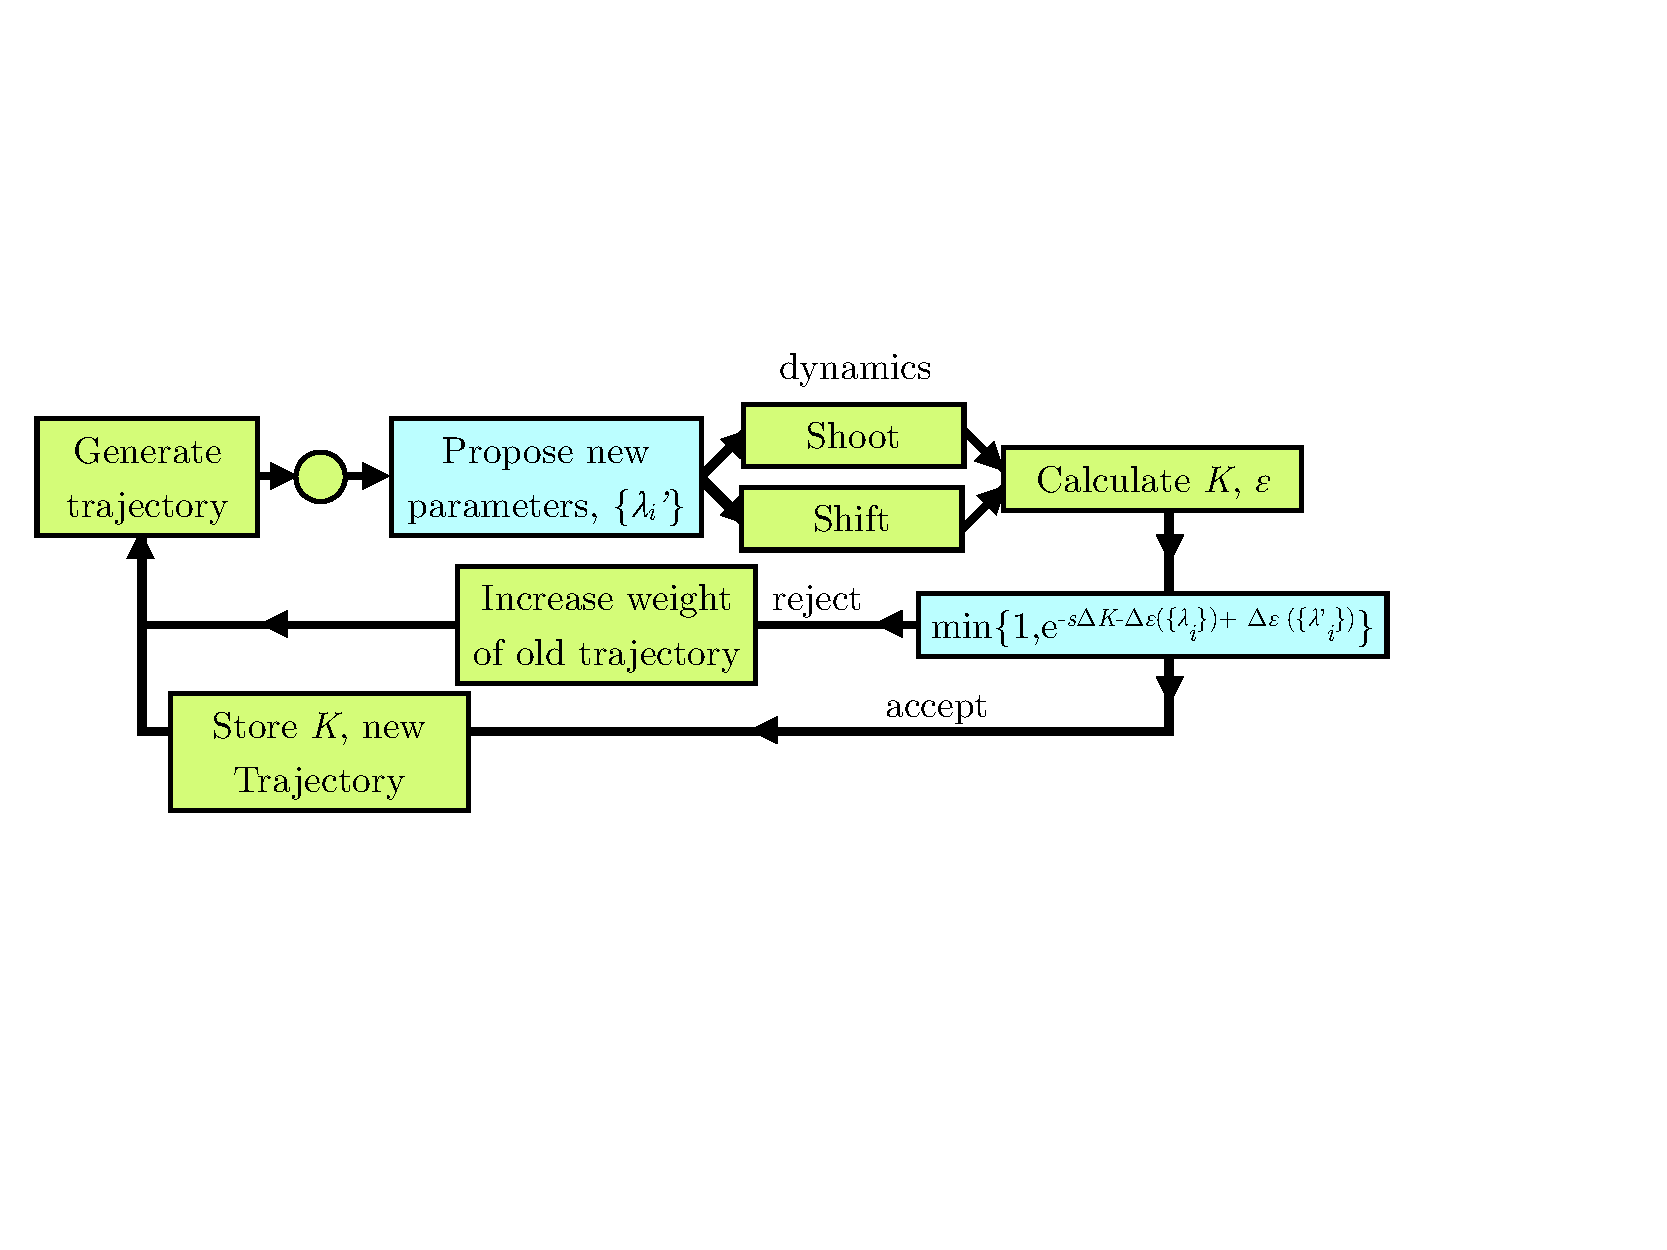
\includegraphics[width=5in]{flowchart.pdf} 
%   \caption{Flow diagram for proposed dynamic tempering algorithm.  Blue boxes indicate steps which are significantly different from the usual TPS scheme with dynamic order parameter, $K$, and field, $s$. Shooting and shifting are the elementary moves of perturbing trajectories in TPS \cite{Bolhuis_AnnuRevPhysChem_2002}.}
%   \label{fig:flow}
%\end{figure}




%\section*{First Stage: Probing Parameter Space to Learn About Trajectories}

Tuning interactions until they produce a desirable effect involves developing a method to allow trajectories to explore parameter space. For specific parameters of interest (which characterize, say, a biological system) we can get insight into dynamics by sampling other regions of parameter space.  This allows us to sample not only the most probable values of our ensemble distribution but also the extremes.   %\subsection*{Algorithm}
%\textbf{1}. Choose a parameter set of interest for simulation, $\{\lambda_{1}, \lambda_{2},...,\lambda_{n}\}$.  Here $\lambda_{i}$ represents some control parameter (for example temperature, $T$) of which there are $n$ such parameters.
%\textbf{2}. Equilibrate trajectories for this system using a path sampling method such as TPS, forward flux sampling \cite{Allen2009} or the string method \cite{E2002}. This can include applying a dynamical field $s$ that couples to some extensive, dynamical variable, $K$.
%\textbf{3}. Choose a new set of parameters $\{\lambda_{1}^{\prime}, \lambda_{2}^{\prime},...,\lambda_{n}^{\prime}\}$.
%\textbf{4}. Simulate the trajectory using the dynamics associated with $\{\lambda_{1}^{\prime}, \lambda_{2}^{\prime},...,\lambda_{n}^{\prime}\}$.

%\textbf{5}. Accept-or-reject these trajectories based on the criterium:
%\begin{align*}
%P_{\mathrm{acc}}&=\min\left \{1,e^{-s \Delta K} \frac{P(\vec{X}^{\prime}|\{\lambda_{1}, \lambda_{2},...,\lambda_{n}\})}{P(\vec{X}|\{\lambda_{1}, \lambda_{2},...,\lambda_{n}\})} \cdot  \frac{P(\vec{X}|\{\lambda_{1}^{\prime}, \lambda_{2}^{\prime},...,\lambda_{n}^{\prime}\})}{P(\vec{X}^{\prime}|\{\lambda_{1}^{\prime}, \lambda_{2}^{\prime},...,\lambda_{n}^{\prime}\})} \right \}
%\end{align*}
%Here, the first factor is the dynamical order parameter equivalent to accepting trajectories based on changes in the dynamical variable $K$ at fixed $\{\lambda_i\}$. This fraction represents the relative weight of the two trajectories in the biased ensemble with field strength $s$.   $P(\vec{X}|\{\lambda_{1}, \lambda_{2},...,\lambda_{n}\})$ is the probability of observing a trajectory $\vec{X}$, a collection  of configurations at various time points $\vec{X}=\{\vec{x},\vec{x}_{1},...,\vec{x}_{N}\}$ given a certain set of parameters $\{\lambda_{1}, \lambda_{2},...,\lambda_{n}\}$. %Here we note that the fraction of the ratios of the initial trajectory ($\vec{X}$) and the new trial trajectory ($\vec{X}^{\prime}$) is the same as the exponential of the negative of the change in action, $\mathcal{E}$, of the trajectory:
%$$ \Delta \mathcal{E}(\vec{X} \rightarrow \vec{X}^{\prime}|\{\lambda_{1}, \lambda_{2},...,\lambda_{n}\}) =  - \ln \left [  \frac{P(\vec{X}^{\prime}|\{\lambda_{1}, \lambda_{2},...,\lambda_{n}\})}{P(\vec{X}|\{\lambda_{1}, \lambda_{2},..\lambda_{n}\})}  \right]$$
%\textbf{6}. Repeat process from step 3. A flow diagram for this process is given in Figure \ref{fig:flow}.

%\subsection*{Test Cases for the First Stage: KCMs}
%To test the effectiveness method,  I will use kinetically constrained models of glass formers.  Specifically, I will test the method using the East \cite{Ritort_AdvInPhys_2003} and the FA model using a trajectory biasing field, $s$.  While the 1d FA model has been well characterized \cite{Garrahan_JPhysA_2008, Elmatad_PNAS_2010}, the hierarchical East model has not been studied in the context of a dynamical phase transition and studying the nature of this expected transition would add new knowledge to the field.  Since the theory \cite{Garrahan2003} which has successfully predicted glass universality~\cite{Elmatad2009} is based on hierarchical modelsthis phase transition is of particular interest. 

%\section*{Second Stage: Using Trajectory Space to Optimize Parameters}
%\begin{figure}[b!] %  figure placement: here, top, bottom, or page
 %  \centering
  % 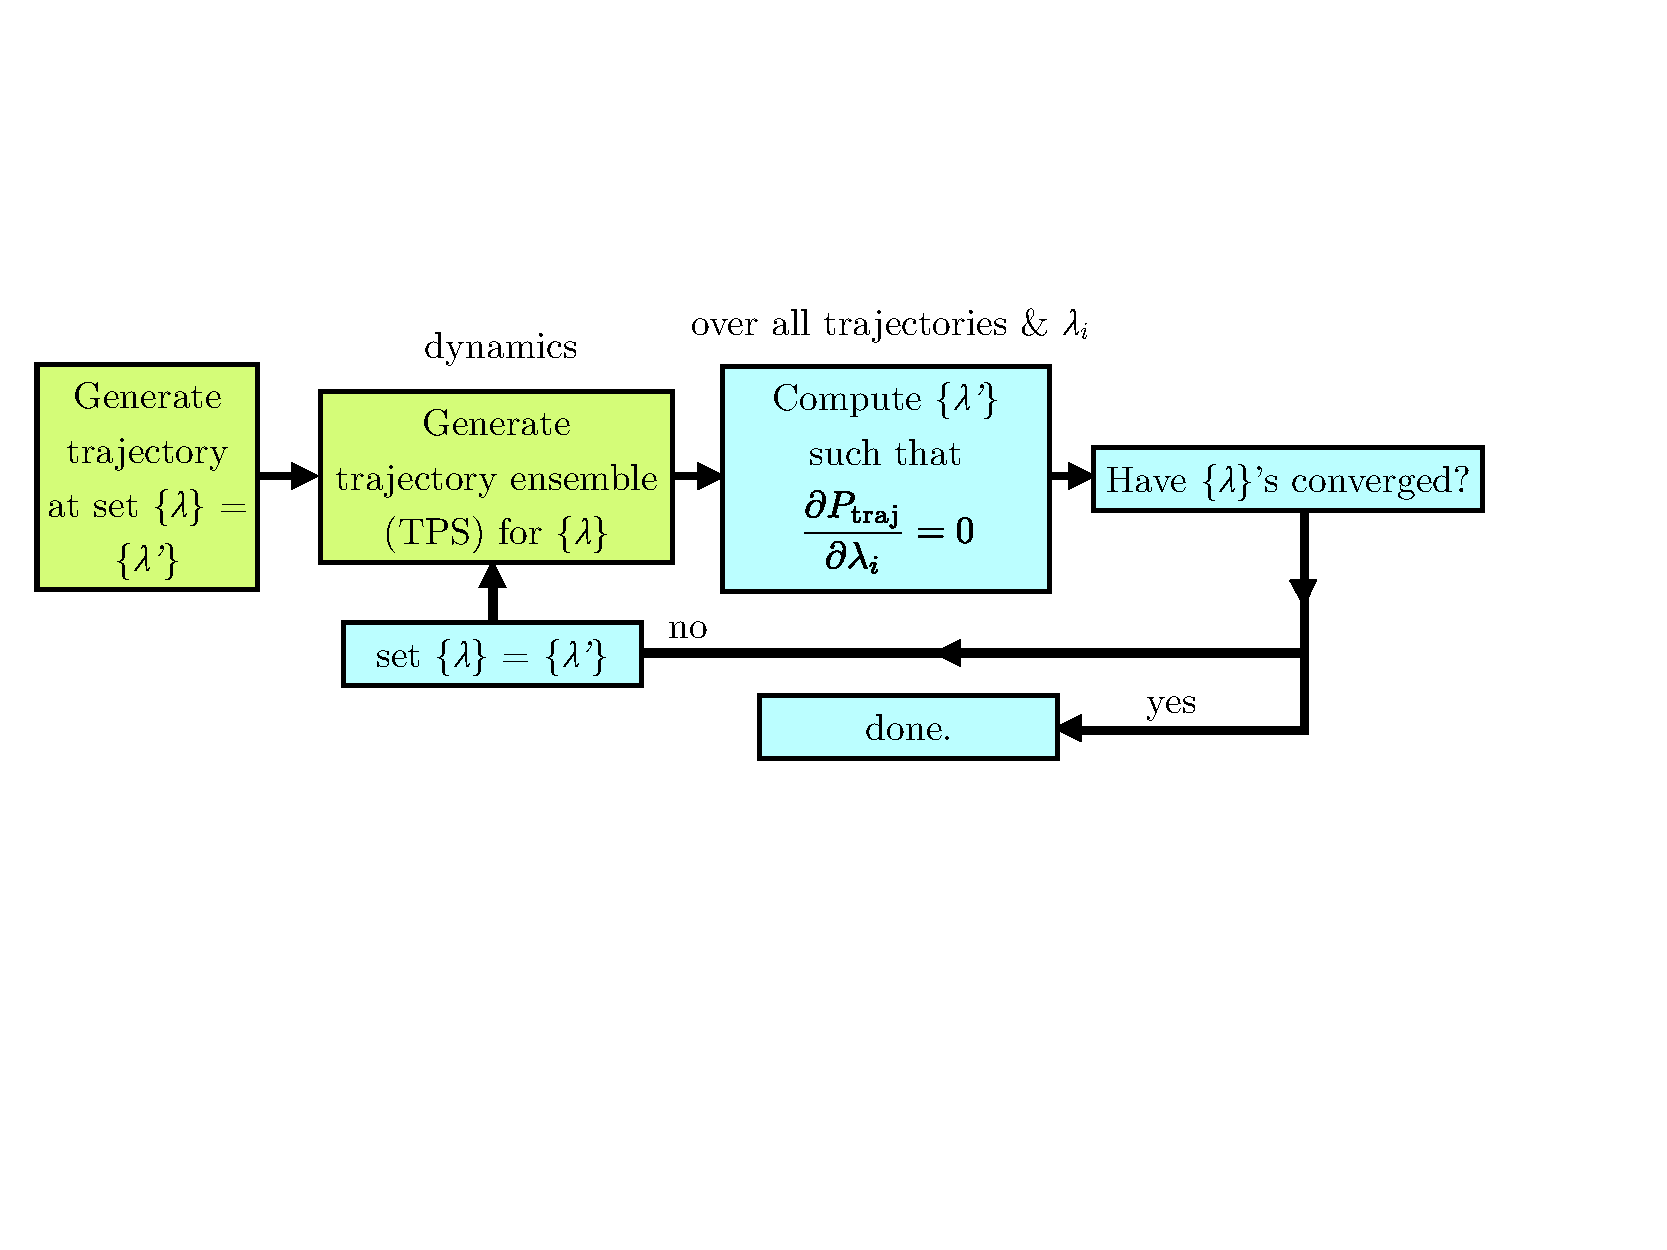
\includegraphics[width=5in]{flowchart_part2.pdf} 
  % \caption{Flow diagram for second phase.  Blue boxes indicate departures from usual transition ensemble harvesting methods.}
   %\label{fig:flow2}
%\end{figure}


Once this information is gathered, I use an ensemble of trajectories to optimize parameters that select for a particular behavior in a system with two basins, $A$ and $B$.  An example of such a system would be a self-assembly process where $A$ is an unassembled state and $B$ is an assembled state.  We seek to optimize the probability of seeing a trajectory that goes from $A$ to $B$ given that the trajectory starts in $A$; that is, optimize, relative to the thermodynamic parameters, the probability of ending in state $B$ given that the system started in state $A$.

%\subsection*{Algorithm}
%\textbf{1}. Generate an ensemble of trajectories that go from $A$ to $B$ in an initial parameter space $\{\lambda_{1}, \lambda_{2}, .. \lambda_{n}\}$.  An example could be the interaction strength between particles.  For each trajectory $\vec{X}$ the probability is given by:
%$$P (\mathrm{\vec{X}}|\{\lambda_{i}\})= P_{0}(\vec{x}_{0}|\{\lambda_{i}\}) \prod_{t=0}^{t_{\mathrm{obs}}} p\left(\vec{x}(t |\{\lambda_{i}\}) \rightarrow \vec{x}(t+\Delta t | \{\lambda_{i}\})\right) $$
%Where $P_{0}(\vec{x}_{0}|\{\lambda_{i}\})$ is the probability of the initial configuration $\vec{x}_0$ and involves estimating the partition function of the system.  $p\left(\vec{x}(t| \{\lambda_{i}\}) \rightarrow \vec{x}(t+\Delta t|\{\lambda_{i}\})\right)$ is the probability of taking a step from configuration $\vec{x}(t| \{\lambda_{i}\})$ at time $t$ to configuration $\vec{x}(t+\Delta t| \{\lambda_{i}\})$ at time $t+\Delta t$ which is parameterized by the current parameter set $\{\lambda_{i}\}$.
%\textbf{2}. Given a set of trajectories, calculate the values of $\{\lambda_{i}\}$ for which these trajectories are most probable. First compute\footnote{In principle, one would really try to maximize the logarithm of $P (\mathrm{\vec{X}}|\{\lambda_{i}\}) $ for computational convenience.  Moreover, one would do this over all values of $\lambda$ as well over the entire ensemble of trajectories.}, $\partial P (\mathrm{\vec{X}}|\{\lambda_{i}\})/\partial \lambda_{i}$.
%For systems on a lattice with simple thermodynamics or systems with Langevin dynamics \cite{IMSM} whose initial conditions do not depend on $\{\lambda_{i}\}$ (say, because particles are too far apart to interact)\footnote{This avoids an expensive calculation of the equilibrium partition function contained in $P_{0}$.}, expressions for these derivatives can be analytically derived in a straightforward manner.    
Optimization methods for these kinds of problems have been recently promoted and are generally referred to as ``maximum likelihood estimators''. %\cite{Crooks2007, Shirts2008, Minh2009}  
These methods can be then used iteratively until an ideal set of parameters is found that increases the probability of going from $A$ to $B$.  This method would act as a kind of conjugate-gradient method for path probability in parameter space.  These results can be informed by real thermodynamic control parameters that experimentalists can actually tune -- such as the interaction strength between particles (experimentally, say, by changing the solvent or tuning some magnetic field).
%.  Use one of these methods to solve for: $\partial P (\mathrm{\vec{X}}|\{\lambda_{i}\})/\partial \lambda_{i} = 0$.
%\textbf{3}. Adopt these new parameters, $\{\lambda_{i}'\}$, and return to step 1.
%\textbf{4}. Repeat process until the parameters $\{\lambda_i\}$ have converged within a given tolerance.  A flow diagram for this process is given in Figure \ref{fig:flow2}.
%\subsection*{Test Cases for Second Stage: Self-Assembly}
%To test this method, I will investigate self-assembly of Janus particles using Brownian dynamics \cite{Jiang2007}.  Janus particles have two opposing faces. For example, one side can be hydrophobic and the other hydrophilic.  These particles can have varied shapes, interaction strengths, and relative compositions and may be useful for technology such as optics \cite{Glotzer2007}.  Tuning these parameters to give specified structures (for example, strings, bilayers, or vesicles) would be a valuable way to determine how parameters play into dynamical pathways. 

%\section*{Long Term Goals}
%These methods would help us understand the link between parameter and trajectory space.  For glass formers, I plan to investigate the links between biased trajectory ensembles and driven systems \cite{Speck2010}. Such connections are tantalizing because they are essential to the idea of facilitation. This would suggest that a link between a biasing field, $s$, in trajectory space and an experimentally measurable system can be found.  In the long term, I hope to use these methods to study the properties of dynamic facilitation since the methods will make simulating complex models more computationally feasible. My other goal is to  design novel materials by understanding self-assembly optimization - such as in the formation of Janus particles into various ordered structures \cite{Glotzer2007}.   The potential to design materials which preform a specified function but whose optimal parameters are not known {\it a priori} is one of the holy grails of theoretical research.  I hope these two methods - and the understanding which comes from employing them - will help make significant advancements in these fields, allowing me to add an increased understanding of the interplay between dynamics and thermodynamics to the scientific community.
%\bibliography{library}

%\bibliographystyle{Science}

\end{document}  
